\chapter{Sprint 3: Uni-carpool}



\section*{Introduction}

\addcontentsline{toc}{section}{Introduction}

In this chapter, we'll be exploring the last Sprint, which focuses on the design and implementation of uni-world's carppoling features.

\section{Sprint Backlog}
To start, we outline the work to be done in this sprint. The schedule for this iteration
involves the user stories described in the following Table 5.1:

\begin{longtable}{|l|p{6cm}|p{8cm}|}
\hline
ID & User story & Task\\
\hline
\endfirsthead

\multicolumn{3}{c}{{\bfseries}} \\
\hline
Sprint & User story & Task\\
\hline
\endhead

\hline \multicolumn{3}{|r|}{{Continued on next page}} \\ \hline
\endfoot

\hline
\endlastfoot
13 & As a student, I want to browse available carpooling offers & \begin{itemize}
    \item Create the Carpool offer model
    \item Create the algorithm responsible for showing the offers
    \item Create the matching system
    \item Create the Carpool feed UI
    \item Integration and testing
\end{itemize} \\ \hline

14 & As a student, I want to show my interest if I find an offer interesting, and ignore offers I don’t like & \begin{itemize}
    \item Creation of like and dislike features
    \item enhancing the algorithm
    \item Integration and testing
\end{itemize} \\ \hline

15 & As a student, I want to create a carpool offer & \begin{itemize}
    \item Creation of messaging UI
    \item Integration and testing
\end{itemize} \\ \hline

16 & As a student, I want to manage my carpool offers & \begin{itemize}
    \item Creation of the carpool management UI
    \item Integration and testing
\end{itemize} \\ \hline

17 & As a student, I want to see who’s interested in my offers & \begin{itemize}
    \item Creation of likes UI 
    \item Integration and testing
\end{itemize} \\ \hline

18 & As a student, I want to accept or reject other users interested in my offers & \begin{itemize}
    \item enhancing the like and dislike features
    \item Integration and testing
\end{itemize} \\ \hline

19 & As a student, I want to receive notifications when I get a match or message & \begin{itemize}
    \item Creation of notification feature
    \item Integration and testing
\end{itemize} \\ \hline
\caption{Sprint 2 backlog}
\label{Tab: Sprint 2 backlog}
\end{longtable}


\section{ Analysis and conception}
In this section, we illustrate the sprint analysis in a more visual representation using use case diagram for the carpooling features and sequence diagrams of the most highlighted features:
"Offers browsing" and "Offers management".

\subsection{Use case diagram}
\textbf{Refined use case diagram for carpooling features: }
\begin{figure}[H] 
            \centering
            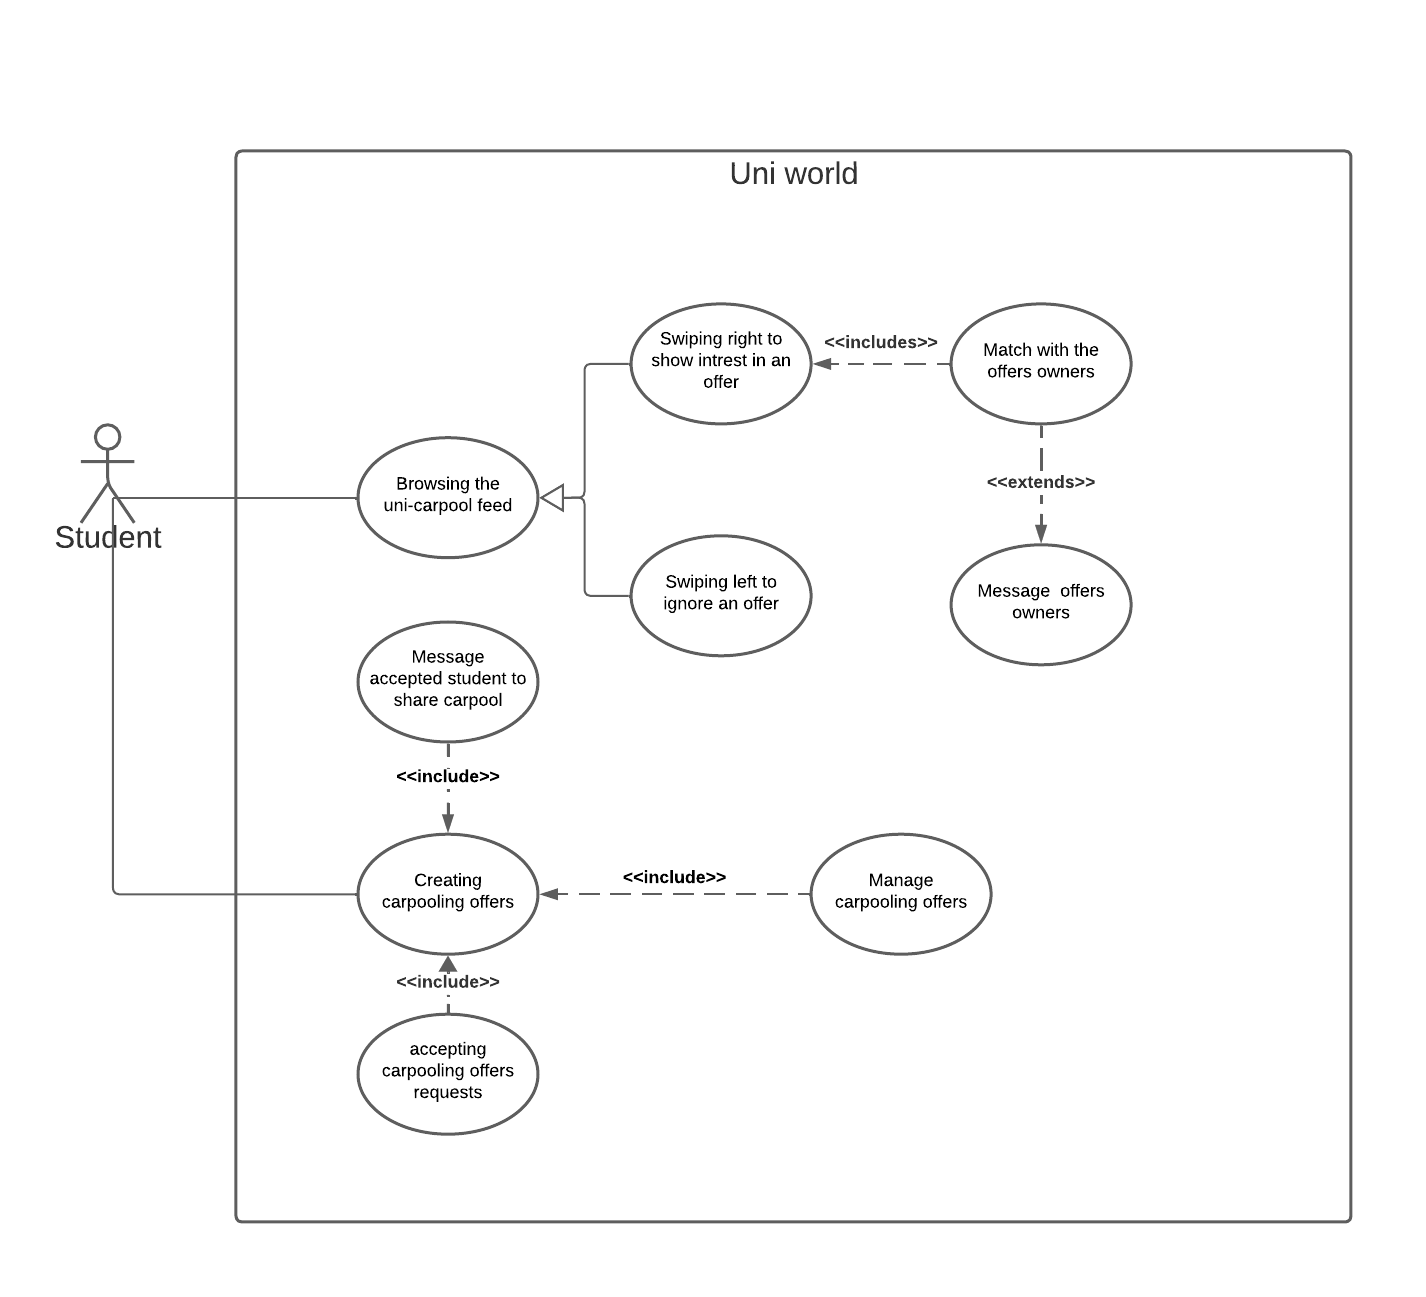
\includegraphics[scale=0.6]{diagrams/refined use case carpool swipe.png}
            \caption{Refined use case diagram for carpooling features} 
            \label{fig: Refined use case diagram for carpooling features}
\end{figure}

\subsection{Use case textual descriptions}
we'll move on to the textual descriptions of the carpooling features such as "Offers browsing" and "Offers management". \\ \\
The offers browsing use case is illustrated in Table 4.2 below:
\begin{longtable}{|c|p{10cm}|}
\hline
Use Case & Description \\\hline
Name & Offers browsing \\\hline
Preconditions & The student must be authenticated and have an active account \\\hline
Post-conditions & once the interest request is accepted by the offer owner, the student and the offer creator match, and a chat will be available to communicate. \\ \hline
Main Flow & 
\begin{enumerate}
    \item After authenticating, the student will get a stack of the offers available in his/her feed.
    \item   Then the student can browse the offer and see information such as the car, the offer owner, the distance between him and the departure place, and both the location of the departure and the arrival places so it helps him/her to choose a suitable offer.
    \item Then the student will have two options:
        \begin{itemize}
            \item   Showing interest in the offer by swiping right on it so that interest can reach the offer owner as a request.
            \item Rejects the offer by swiping left on it to ignore it and move to other options simply.
        \end{itemize} 
        \item The action will be incorporated into the system. 
\end{enumerate}
\\\hline
Alternative Flows & 
    if there is a network error, an error message appears
\\\hline
\caption{Textual descriptions of the Offers browsing use case}
\label{Tab: Textual descriptions of the Offers browsing use case}
\end{longtable}

The use case textual description of "Offers management" is illustrated in the
following Table 3.3:

\begin{longtable}{|c|p{10cm}|}
\hline
Use Case & Description \\\hline
Name & Offers management \\\hline
Preconditions & The student must be authenticated and have an active
account \\\hline
Post-conditions & user A and User B can match if user A likes User B back
\\\hline
Main Flow &
\begin{enumerate}
    \item After logging in, the student will choose to go to the carpool offer management screen.
    \item The student can then browse their offers to see who is interested in them
    \item The student will then have several options
       \begin{itemize}
        \item Accept or reject requests
        \item Modify an offer
        \item Delete an offer
        \item Add a new offer
    \end{itemize} 
\end{enumerate}
\\\hline
Alternative Flows & \begin{itemize}
    \item if there is a network error, an error message appears
\end{itemize}
\\\hline
Non-functional Requirements & \begin{itemize}
    \item The carpooling offers management will have a user-friendly UI
\end{itemize}
\\\hline
\caption{Textual descriptions of the carpooling offers use case}
\label{Tab: Textual descriptions of the carpooling offers use case}
\end{longtable}

\subsection{Sequences diagram}
The carpooling offers browsing object sequence diagram can be observed in Figure 5.3 below:

\begin{figure}[H] 
            \centering
            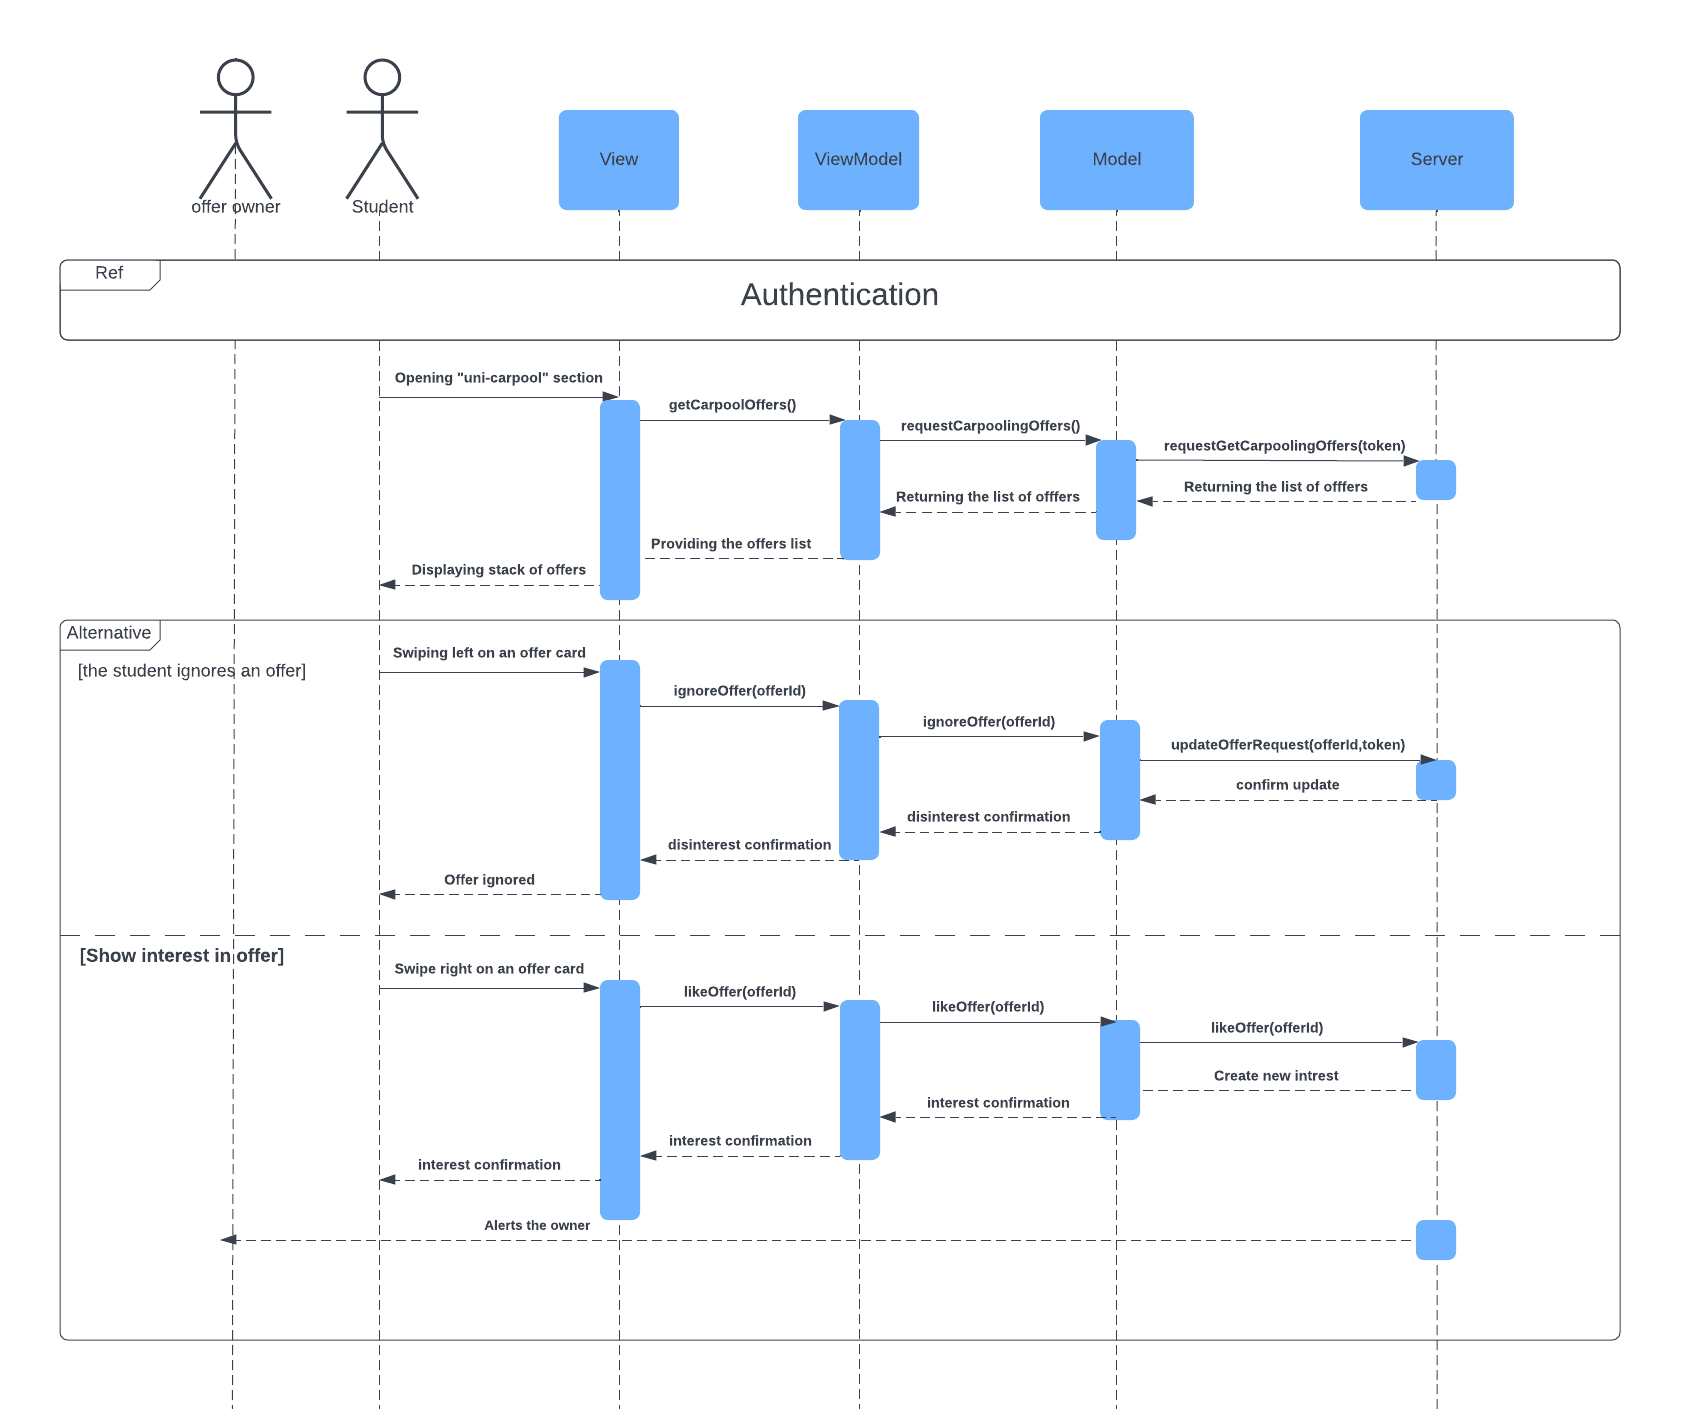
\includegraphics[scale=0.45]{diagrams/Sequence diagram object carpool browsing.png}
            \caption{carpooling offers browsing object sequence diagram} 
            \label{fig: carpooling offers browsing object sequence diagram }
\end{figure}

The adding carpool offers system sequence diagram can be observed in Figure 5.4 below:

\begin{figure}[H] 
            \centering
            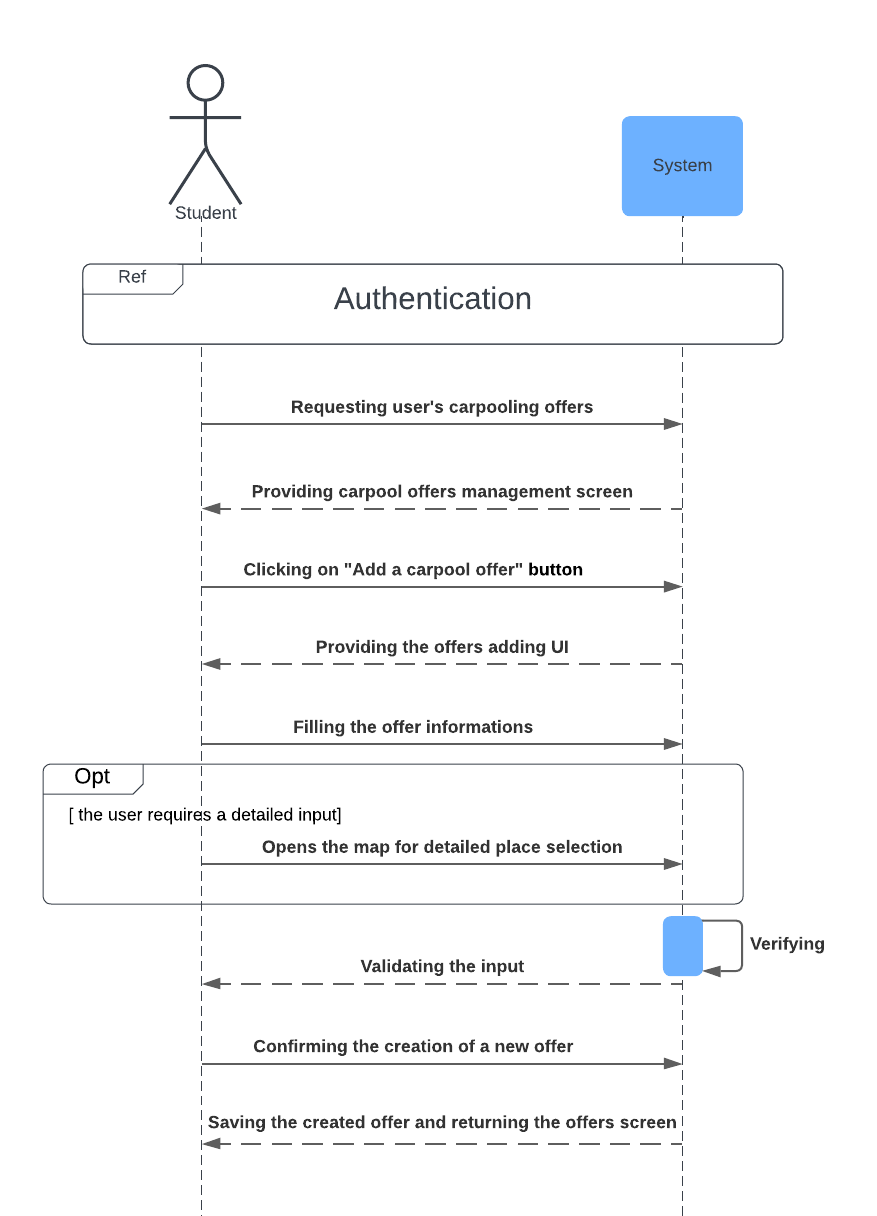
\includegraphics[scale=0.5]{diagrams/Sequence diagram system add carpool offer.png}
            \caption{Add new carpool offer system Sequence diagram } 
            \label{fig: Add new carpool offer system Sequence diagram}
\end{figure}

\section{Realization}
In this section, we describe what has been implemented and how the various components and functionalities identified in this Sprint have been instantiated.

\subsection{Uni-carpool feed and offers browsing}

After taking the user's needs into account, he or she will have a feed full of carpooling offers to choose from, and the user interface will be easy and fun to use, requiring only two main behaviors: scrolling, and swiping. scrolling in this context gives the user the detail view of the offer; and swiping that gives the user the gesture to show interest or ignore the offer.\\

Below, we take a look at the feed where the user can swipe on different offers. \\
\begin{figure}[H] 
            \centering
            \includegraphics[scale=0.1]{ui/unicarpool feed ui.png}
            \caption{Some Uni-carpool feed UIs} 
            \label{fig: Uni-carpool feed UIs}
\end{figure}

\subsection{Adding offers}
Any user can add a new carpool offer, uni-carpool provides an easy-to-use process for adding an offer by submitting details such as departure and destination locations, the price of the journey if the user wishes to earn extra money, the estimated arrival time as well as a description so he can talk more about the offer and finally he can put photos related to the journey to attract other users and make his offer noticeable. \\
In the figure below, we take a look at how we can add a carpooling offer showing the UIs where the user can add his offers
\begin{figure}[H] 
            \centering
            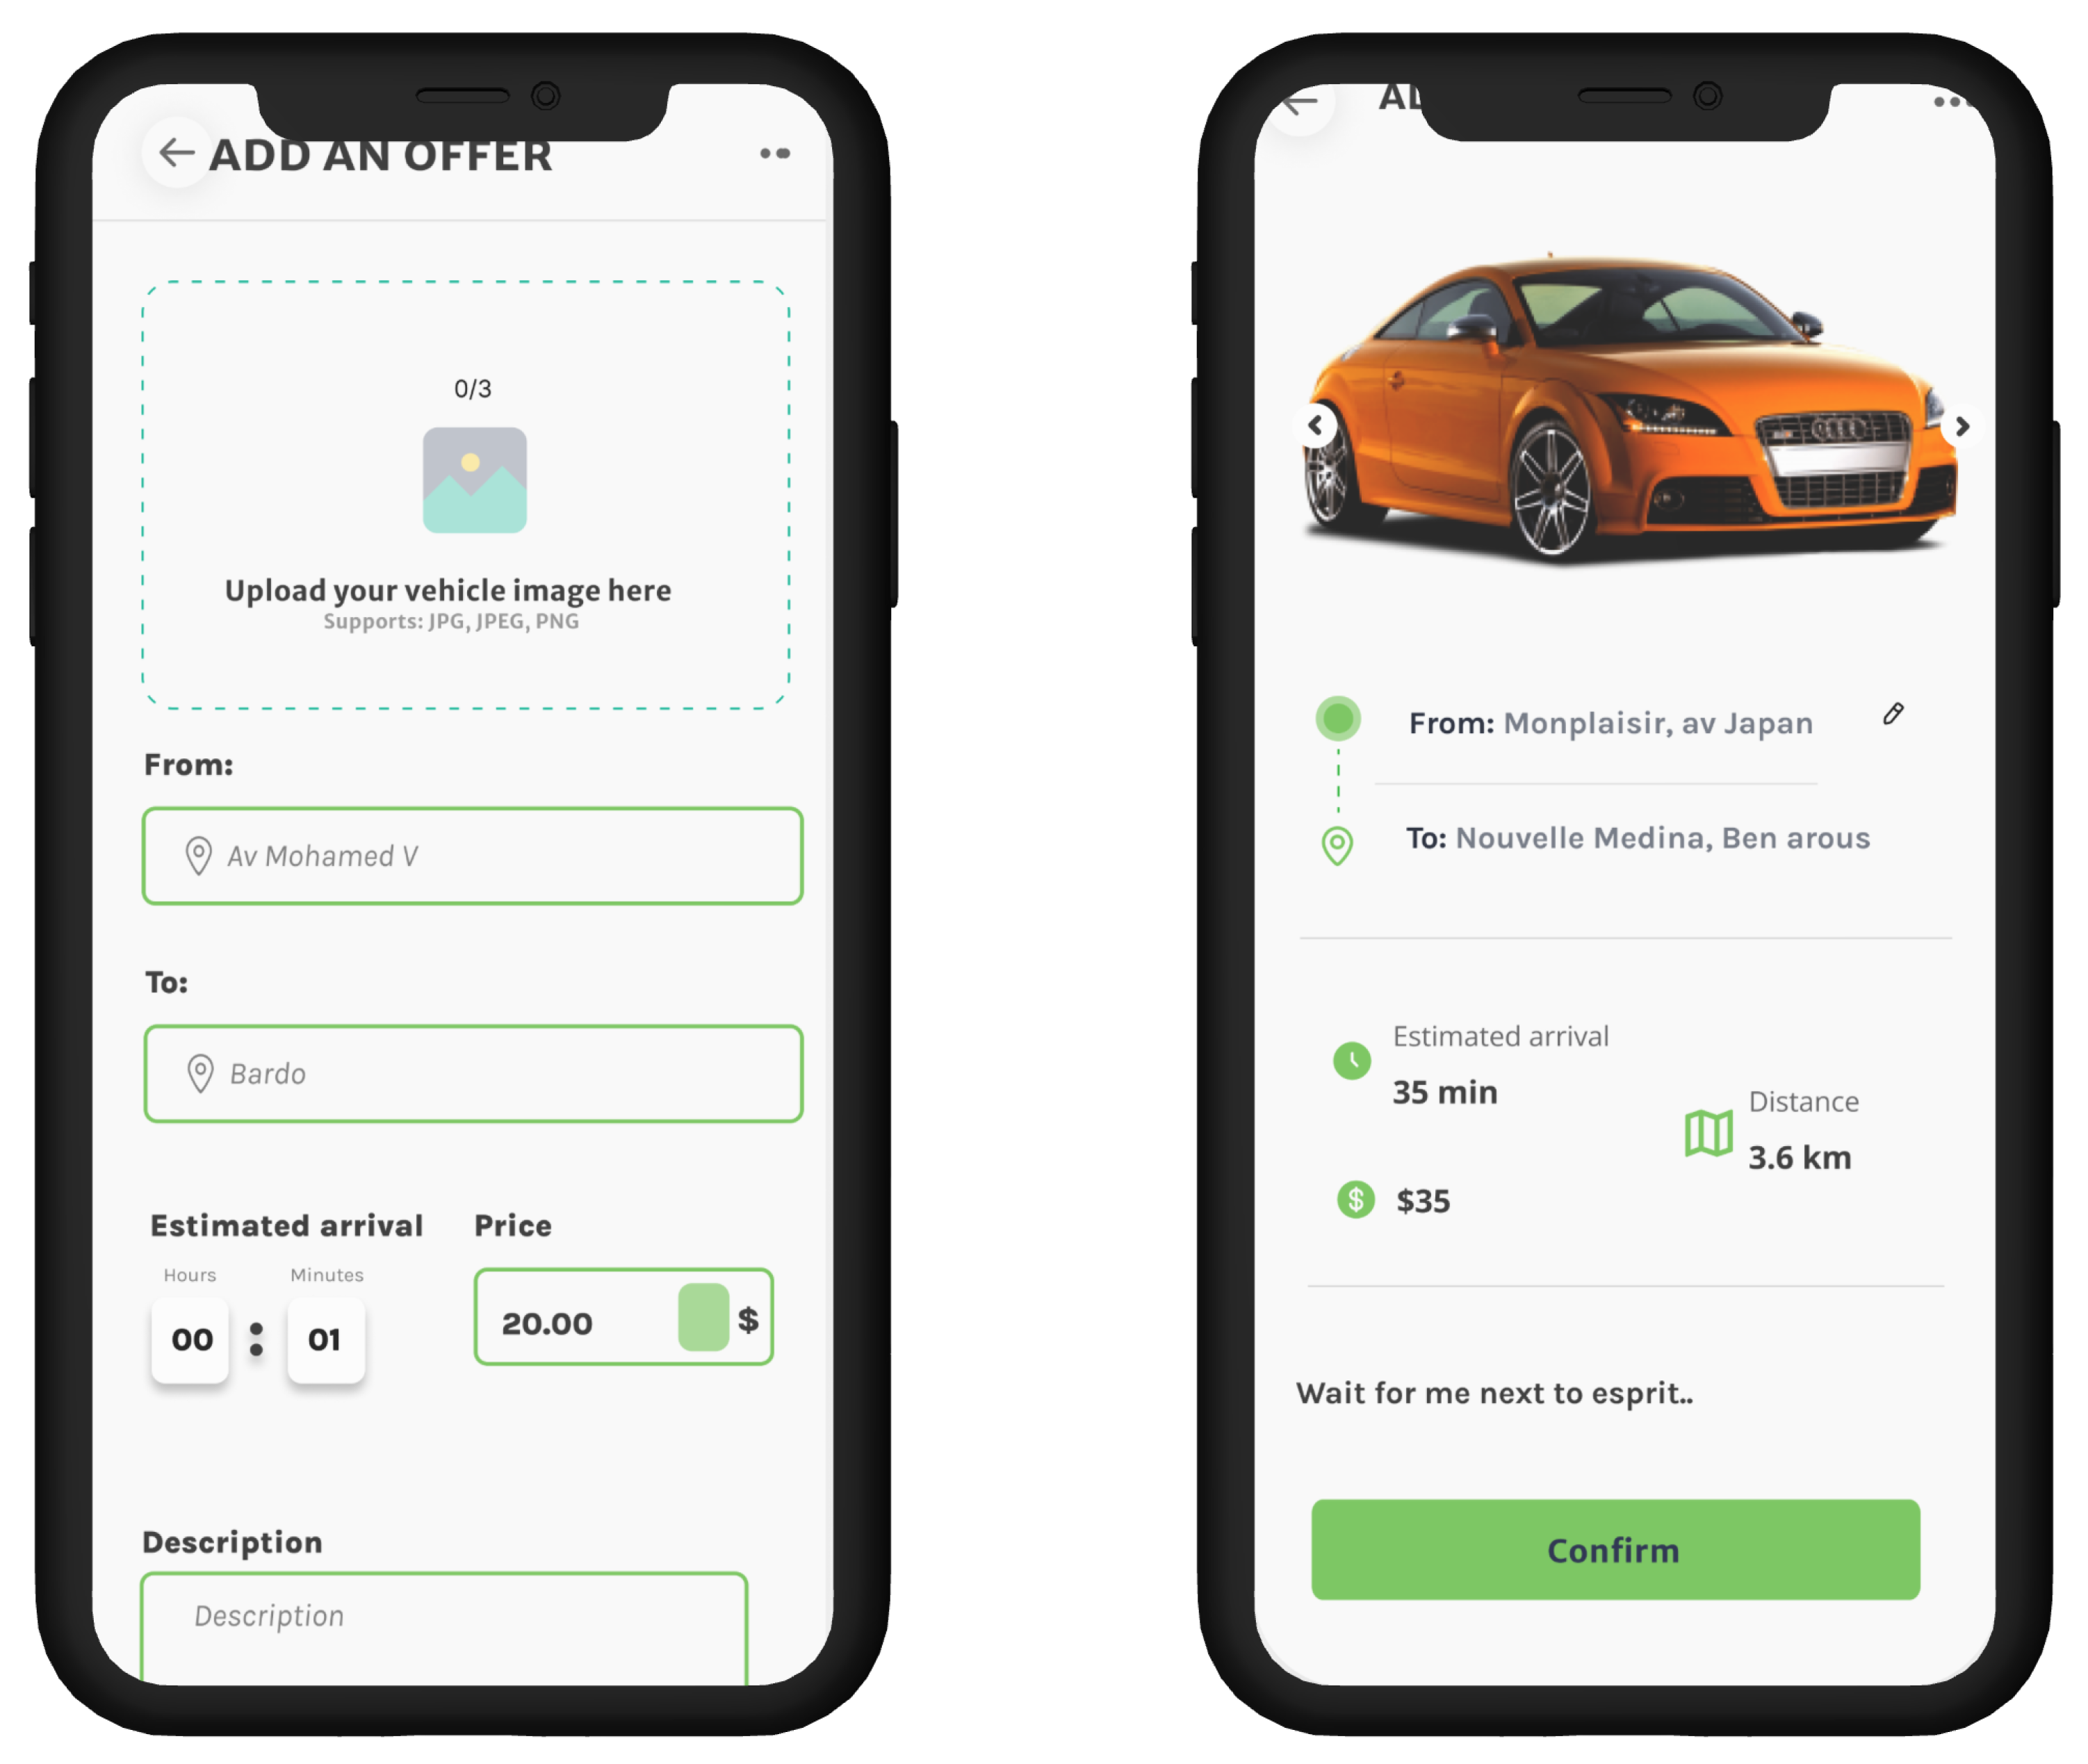
\includegraphics[scale=0.15]{ui/adding carpooling offer.png}
            \caption{Adding carpooling offer feature} 
            \label{fig: Adding carpooling offer feature UI}
\end{figure}

\subsection{Offers management}
What happens after right swiping according to the suggested algorithm is that after right swiping on an offer, the owner of that offer, that is the person who created the offer will notice it in the “Offer management” section. Here users can view the details of people who expressed an interest of their various offers and either approve or deny the request. \\
In the figure below, we take a look at the carpooling offers management screen where the user can manage his offers
\begin{figure}[H] 
            \centering
            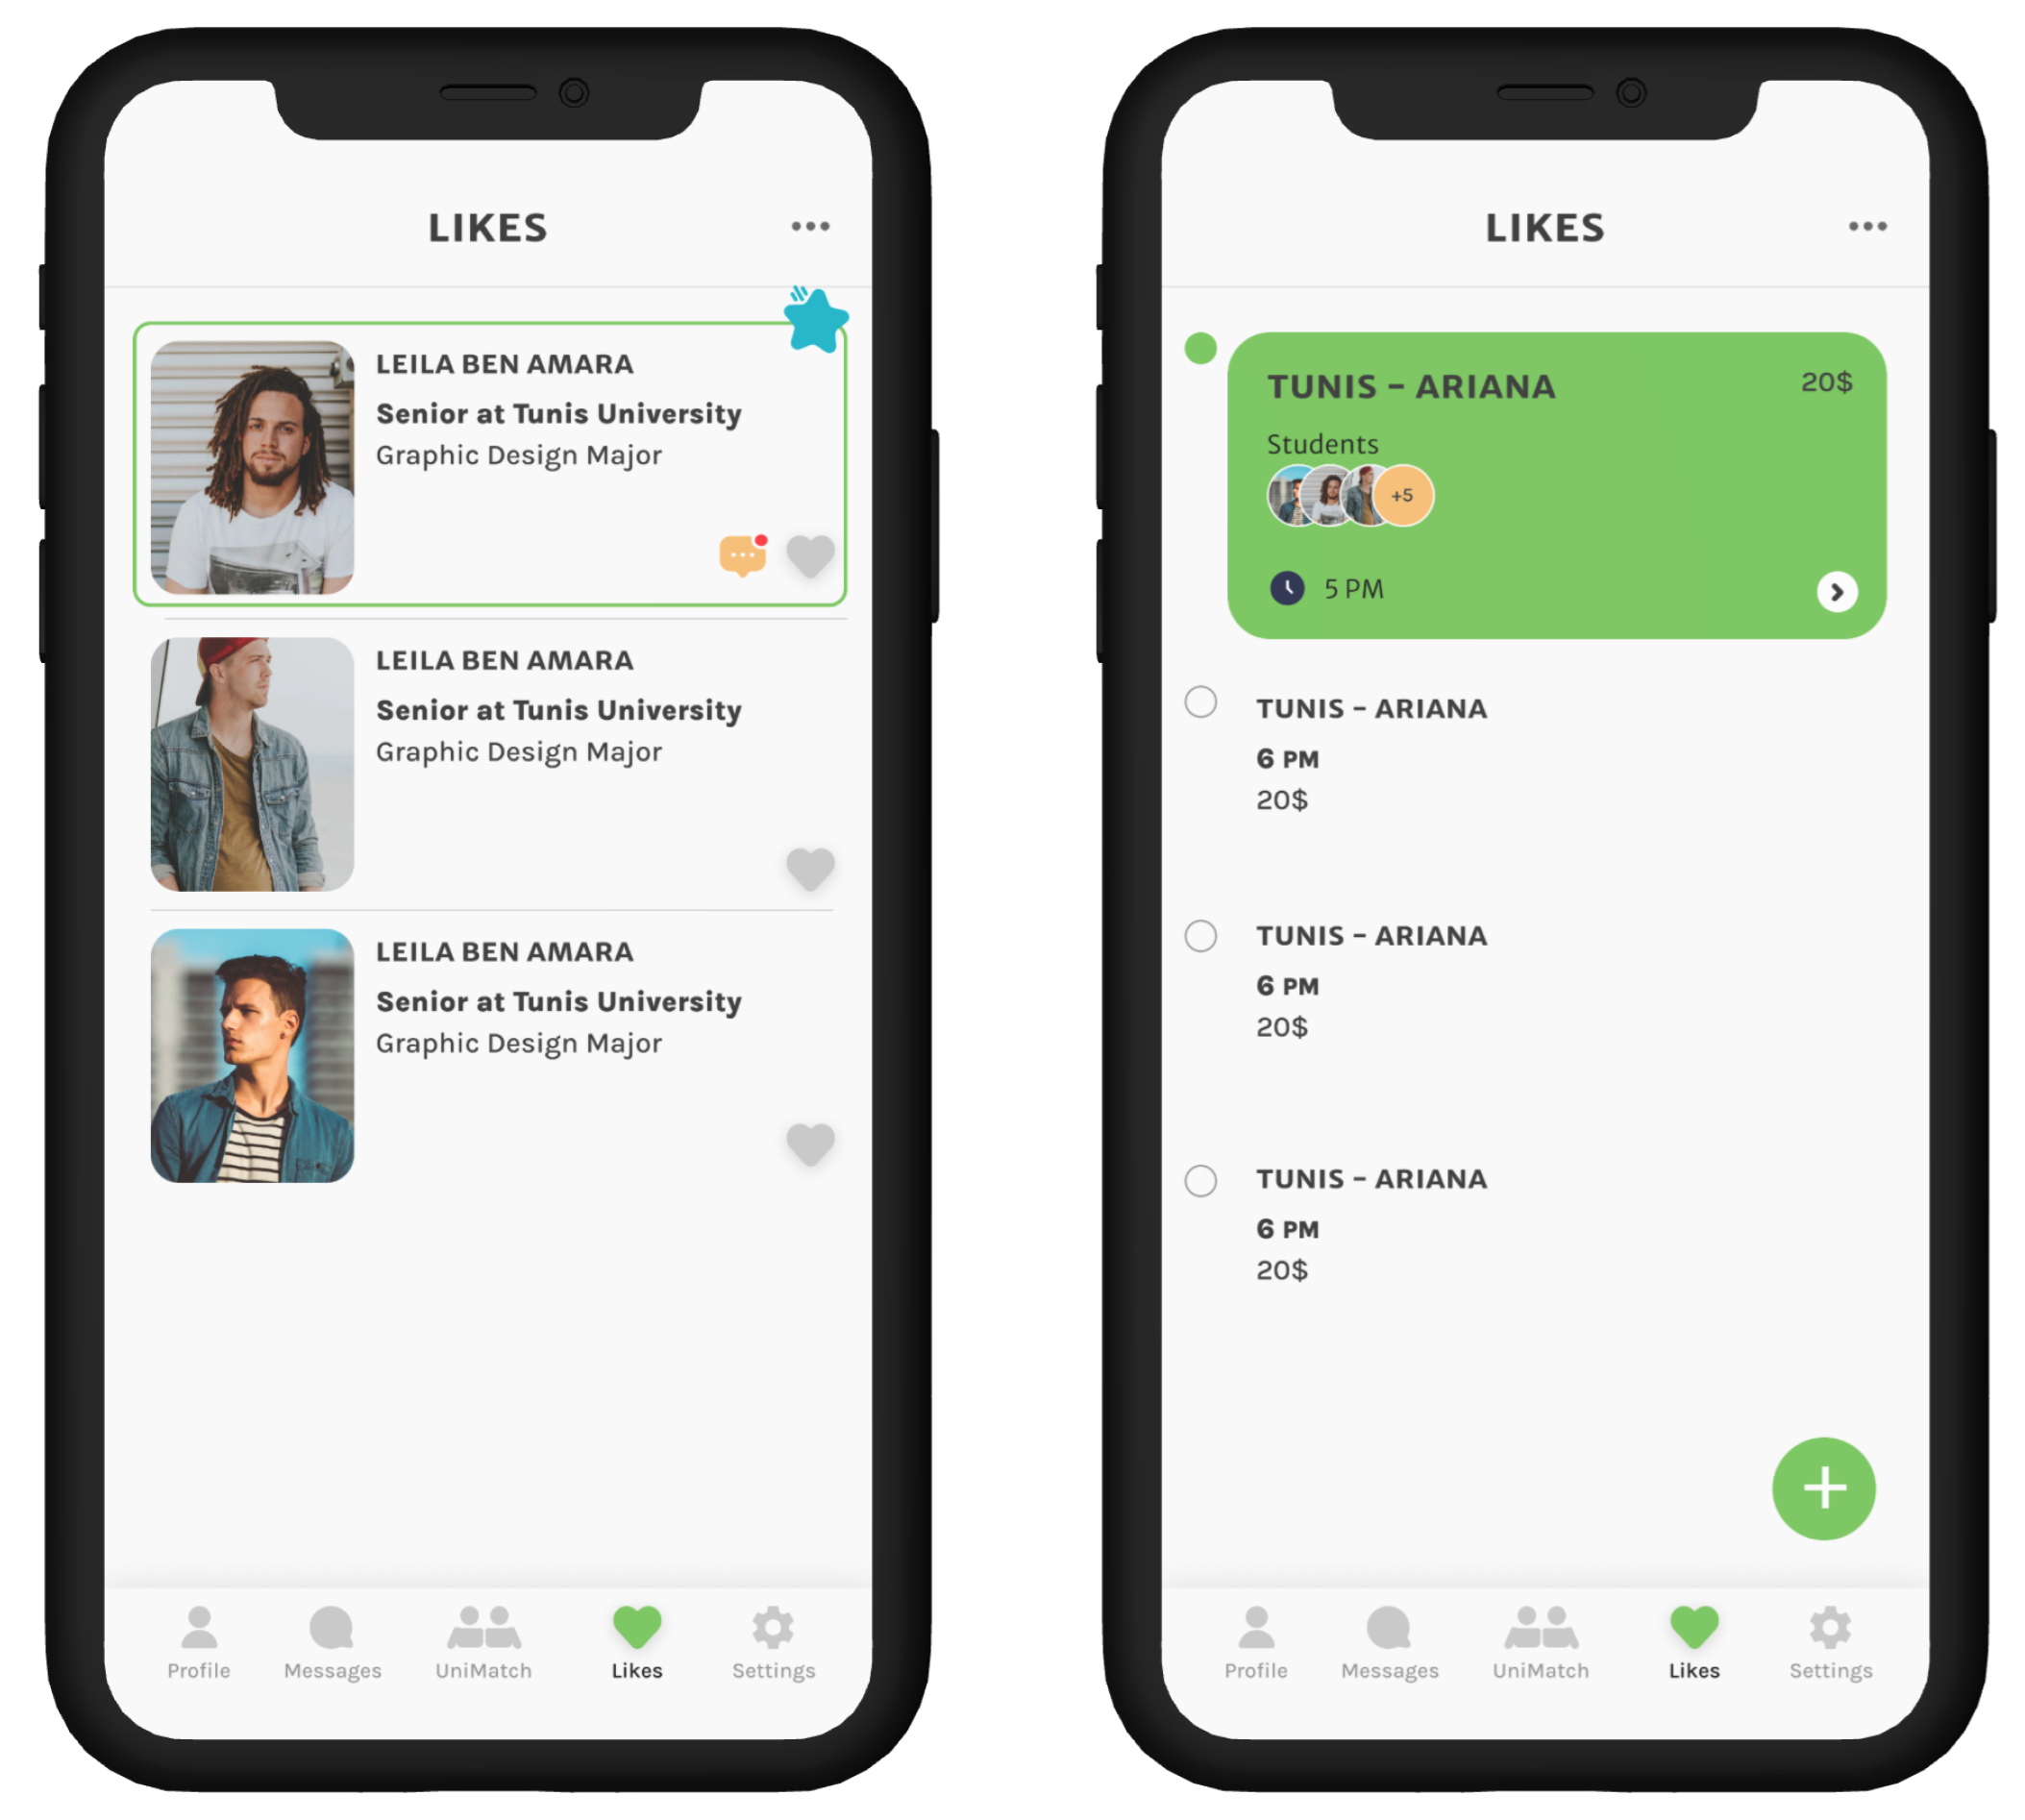
\includegraphics[scale=0.2]{ui/unicarpool offer managment.png}
            \caption{Uni-carpool offers management UI} 
            \label{fig: Uni-carpool offers management UI}
\end{figure}

\subsection{Messaging features}
As stated in the previous subsection, the owner can see who is interested in his offer. He then decides whether or not to decline or approve the sharing request. When he accepts a request, a new conversation is made which allows the sender of the request and the owner of the offer to interact. \\

Below, the direct message user interface is designed to enable users to communicate with one another.
\begin{figure}[H] 
            \centering
            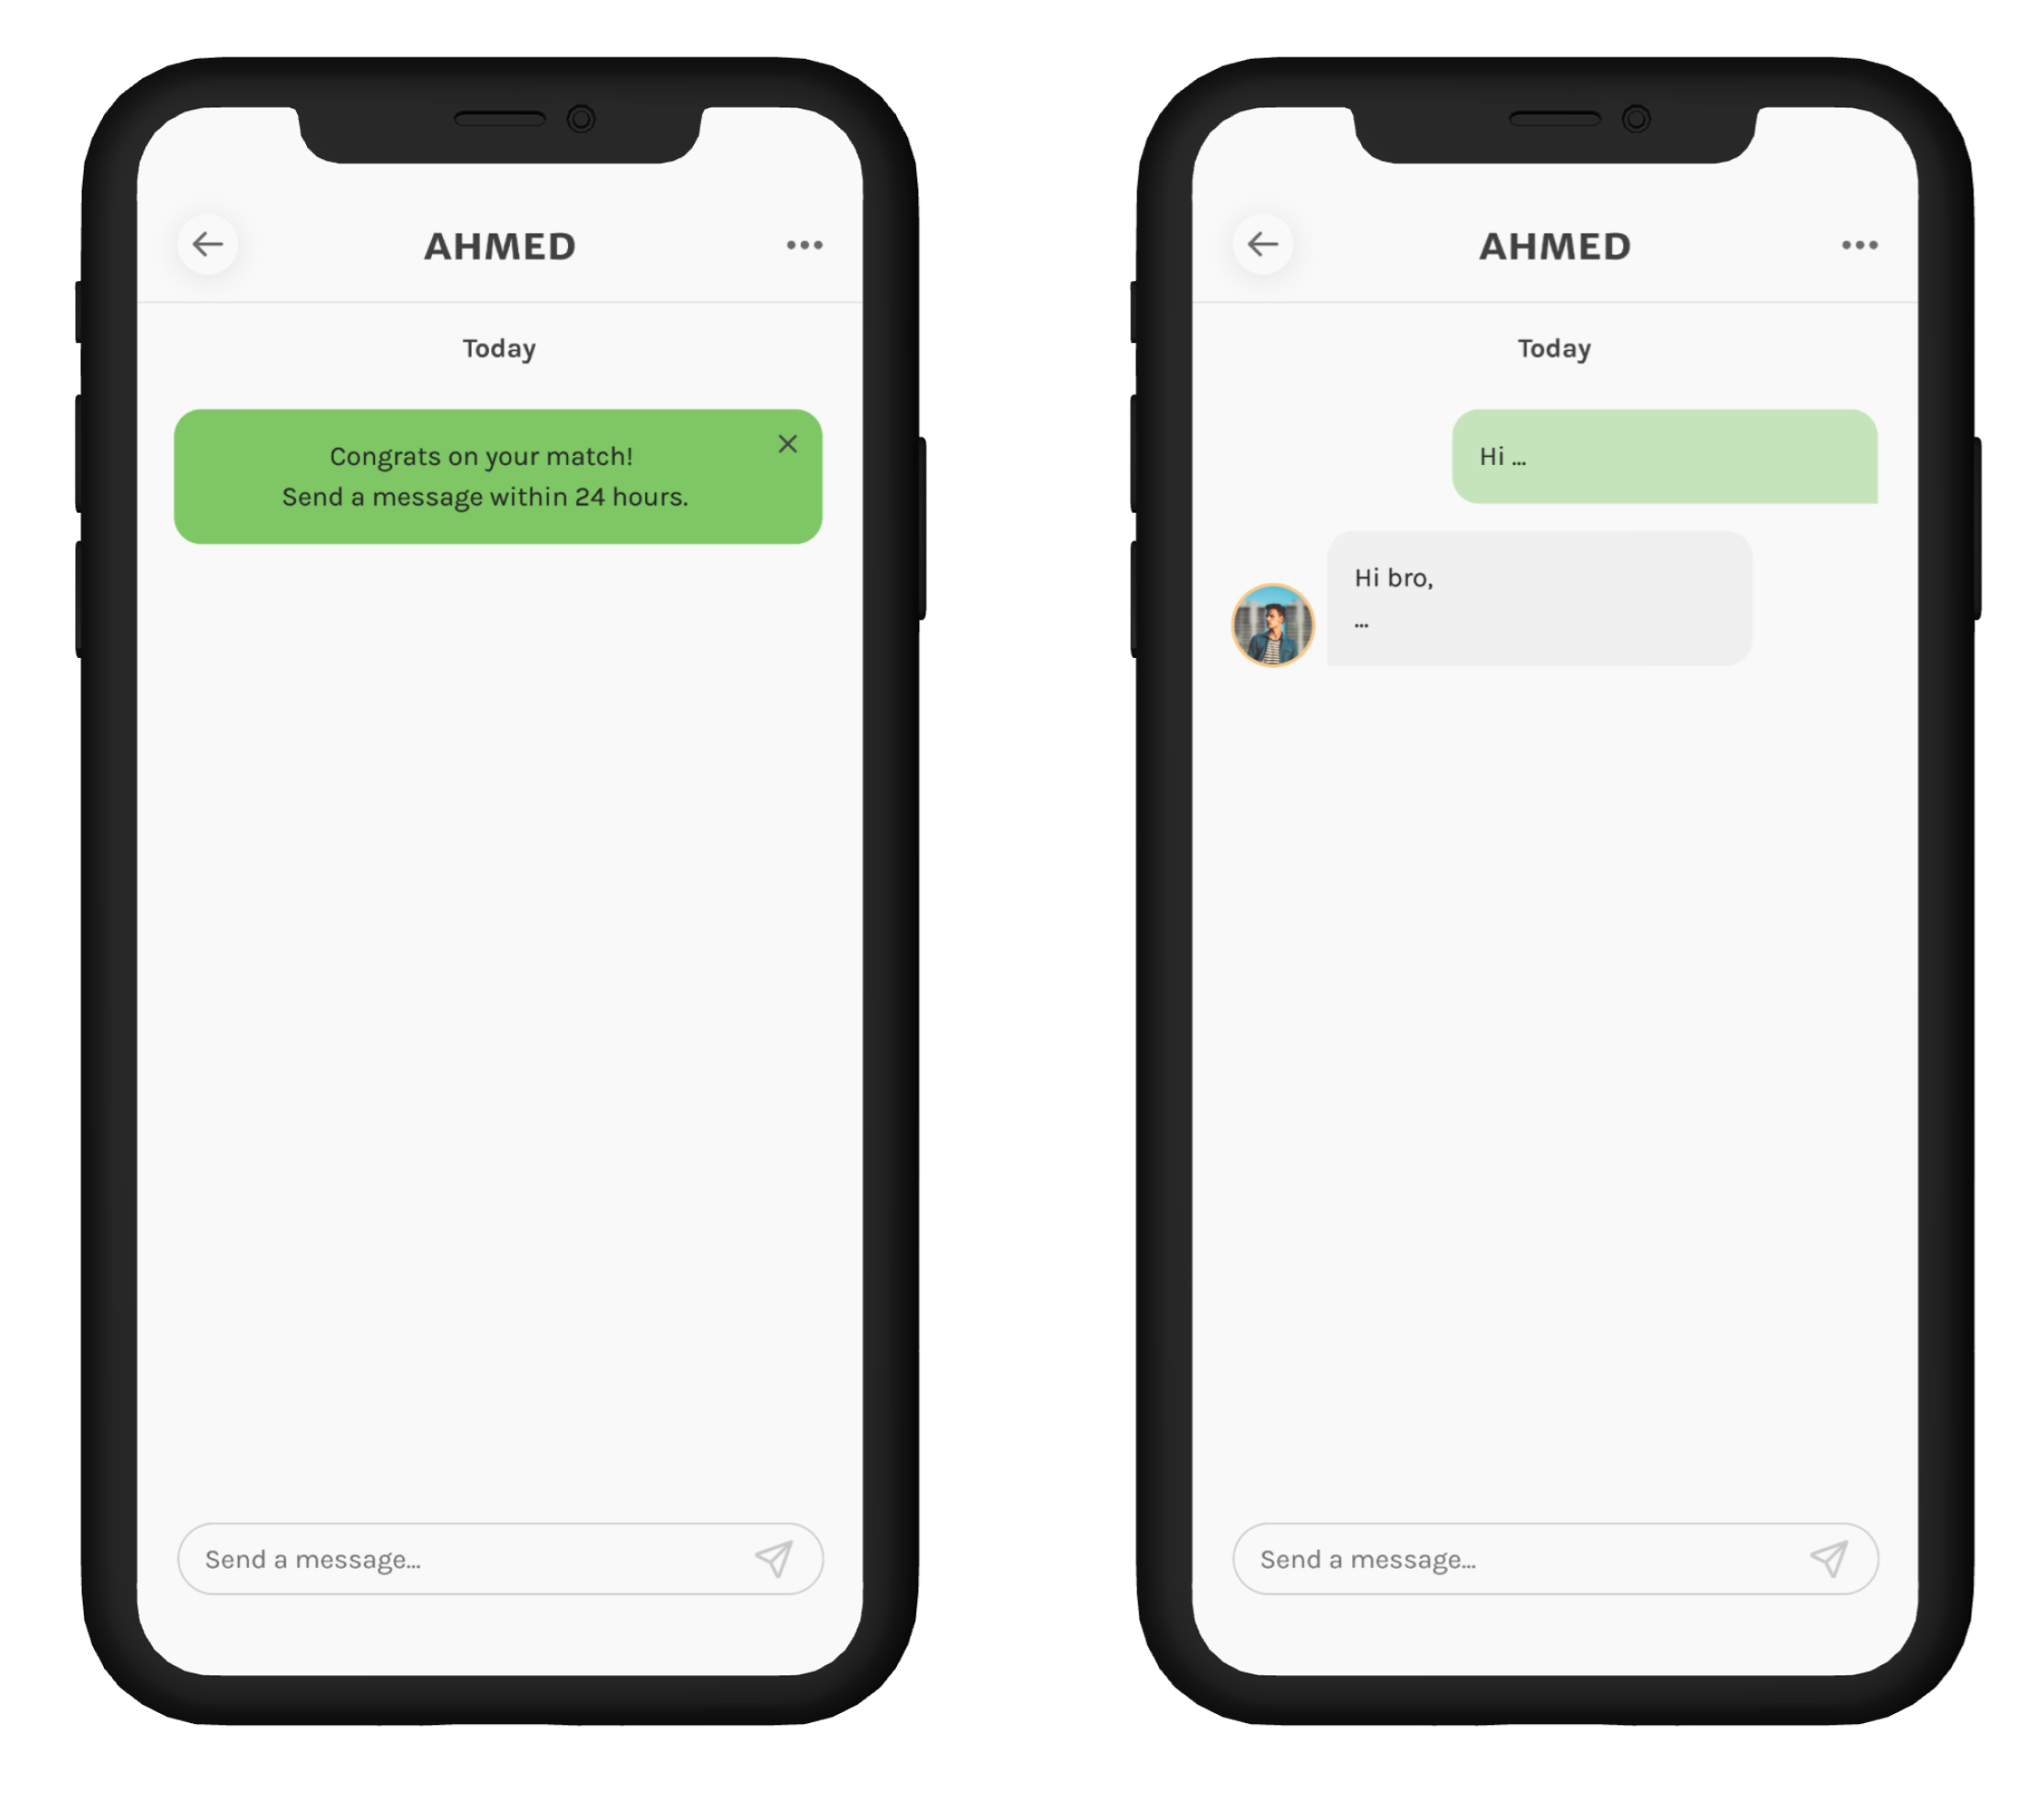
\includegraphics[scale=0.2]{ui/unicarpool messaging.png}
            \caption{Uni-carpool messages UI} 
            \label{fig: messages UI}
\end{figure}

\section*{Conclusion}
\addcontentsline{toc}{section}{Conclusion}
Sticking to the tradition of the chosen methodology, the first sprint introduced a design of the features that are complete for managing users and their authentication. The fact that it is possible to test and specifically these features in the subsequent sprints is the point that brings the team closer to the goal and the great immersive experience. 

